% \documentclass[tikz]{standalone}
\tikzset{
    level/.style = {
        ultra thick,
        black,
    },
    connect/.style = {
        dashed,
        black
    },
    notice/.style = {
        draw,
        rectangle callout,
        callout relative pointer={#1}
    },
    label/.style = {
        text width=2cm
    }
}
% \begin{document}
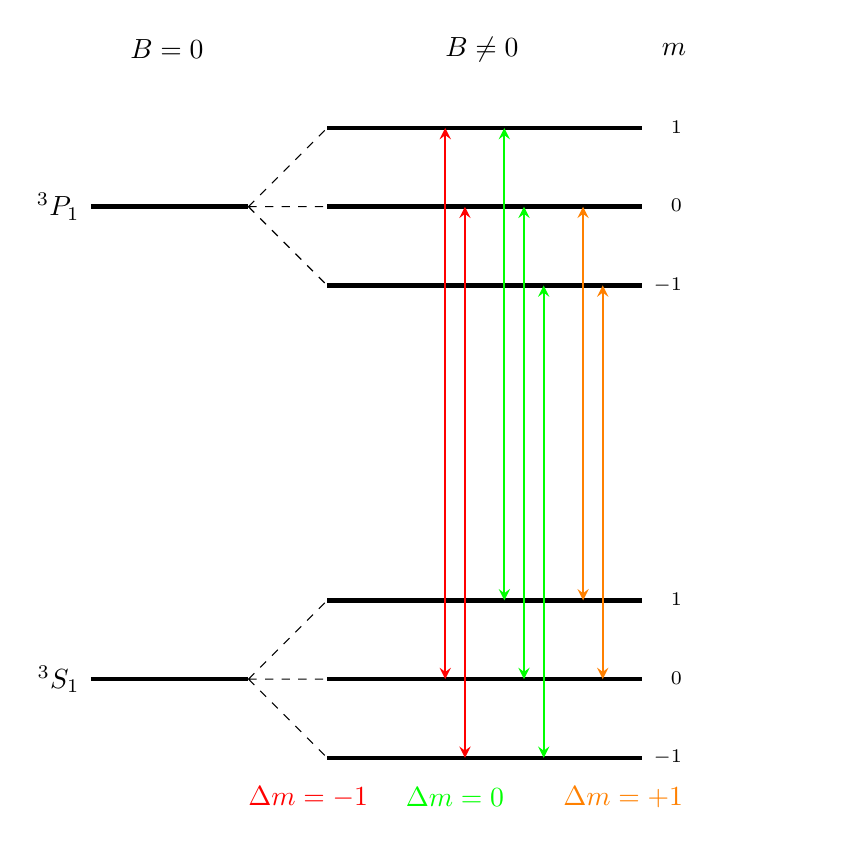
\begin{tikzpicture}
    % Draw all levels
    \draw[level] (0,+3) node[left] {$^3P_1$} -- (2,+3);
    \draw[level] (0,-3) node[left] {$^3S_1$} -- (2,-3);

    \draw[connect] (2,+3) -- (3,+4) (2,+3) -- (3,+3) (2,+3) -- (3,+2);
    \draw[connect] (2,-3) -- (3,-4) (2,-3) -- (3,-3) (2,-3) -- (3,-2);

    \draw[level] (3,+4) -- (7,+4) node[right] {\scriptsize $\phantom{-}1$};
    \draw[level] (3,+3) -- (7,+3) node[right] {\scriptsize $\phantom{-}0$};
    \draw[level] (3,+2) -- (7,+2) node[right] {\scriptsize $-1$};
    \draw[level] (3,-2) -- (7,-2) node[right] {\scriptsize $\phantom{-}1$};
    \draw[level] (3,-3) -- (7,-3) node[right] {\scriptsize $\phantom{-}0$};
    \draw[level] (3,-4) -- (7,-4) node[right] {\scriptsize $-1$};

    % Draw arrows
    \draw [stealth-stealth, thick, red]({4 + 2/4},+4) -- ({4 + 2/4},-3);
    \draw [stealth-stealth, thick, red]({4 + 3/4},+3) -- ({4 + 3/4},-4);
    %
    \draw [stealth-stealth, thick, green]({5 + 1/4},+4) -- ({5 + 1/4},-2);
    \draw [stealth-stealth, thick, green]({5 + 2/4},+3) -- ({5 + 2/4},-3);
    \draw [stealth-stealth, thick, green]({5 + 3/4},+2) -- ({5 + 3/4},-4);
    %
    \draw [stealth-stealth, thick, orange]({6 + 1/4},+3) -- ({6 + 1/4},-2);
    \draw [stealth-stealth, thick, orange]({6 + 2/4},+2) -- ({6 + 2/4},-3);


    % Draw labels
    \node[label] at (1.5,5) {$B = 0$};
    \node[label] at (5.5,5) {$B \neq 0$};
    \node[label] at (8.25,5) {$m$};

    \node[label, red] at (3+0,-4.5) {$\mathrm\Delta m = -1$};
    \node[label, green] at (3+2,-4.5) {$\mathrm\Delta m = 0$};
    \node[label, orange] at (3+4,-4.5) {$\mathrm\Delta m = +1$};
\end{tikzpicture}
% \end{document}
